\documentclass{article}
\usepackage[T2A]{fontenc}
\usepackage[utf8]{inputenc}
\usepackage{hyperref}
\usepackage{graphicx}
\usepackage[english,russian]{babel}
\usepackage{fancyhdr}

%
\usepackage{tabularx}
\usepackage{array}
\usepackage{longtable}
\usepackage{tabularray}
\usepackage{tikz}

% For... glossary
\usepackage[toc,translate=babel]{glossaries}

% To set custom label for enumerate
\usepackage{enumitem}

\usepackage[left=2cm,right=2cm]{geometry}

\author{Егор Федоров \and Андрей Карабанов}
\title{Software Requirements for Zadachnik}

\pagestyle{fancy}
\fancyhead{}
\fancyfoot[C]{\thepage}

\renewcommand{\headrulewidth}{0pt}
\fancypagestyle{firststyle}
{
	\fancyhead{}
	\fancyfoot[C]{г. Санкт-Петербург\\2024 г.}
}


\makenoidxglossaries
\newglossaryentry{task}{
  name={задача},
  description={это минимальная единица работы, которая должна быть выполнена в рамках проекта. В Scrum задачи представляют собой конкретные действия или части работы, требуемые для завершения пользовательской истории или другого крупного элемента, например, тестирования, разработки или исправления ошибки. Каждая задача имеет стату  и может быть назначена одному разработчик.}
}
\newglossaryentry{story}{
  name={стори},
  description={это короткое, простое описание функциональности системы с точки зрения конечного пользователя или клиента. Стори создается для выражения потребности или цели, которые должна удовлетворить команда разработки.}
}
\newglossaryentry{epic}{
  name={эпик},
  description={это крупная пользовательская история или крупный элемент работы, который нельзя выполнить в одном спринте. Эпик обычно разбивается на несколько стори или задач для удобства управления. Он описывает более долгосрочные цели и широкие функции продукта. Эпик может охватывать несколько спринтов или даже несколько версий продукта.}
}
\newglossaryentry{sprint}{
  name={спринт},
  description={это фиксированный отрезок времени (обычно от 1 до 4 недель), в течение которого команда разработки должна выполнить набор задач из бэклога спринта. Спринт начинается с планирования, а заканчивается демонстрацией результата и ретроспективой. Цель спринта — завершить все запланированные задачи и получить инкремент продукта, который можно продемонстрировать стейкхолдерам}
}
\newglossaryentry{product-backlog}{
  name={product backlog},
  description={это упорядоченный и постоянно обновляемый список всего, что планируется сделать для создания и улучшения продукта. Этот артефакт Скрама является единственным источником работы для Скрам-команды. \Gls{product-owner} несет ответственность за Бэклог Продукта, включая его содержимое, доступность и упорядочение}
}
\newglossaryentry{product-owner}{
  name={product Owner},
  description={это одна из 3 зон ответственности в Скрам-команде. Владелец Продукта отвечает за максимизацию ценности продукта, получаемого в результате работы Скрам-команды. В его обязанности также входит курирование и приоритизация Бэклога Продукта. Около 50\% времени Владелец Продукта проводит с клиентами и заинтересованными лицами, остальные 50\% работает совместно с командой}
}
\newglossaryentry{kanban-board}{
  name={kanban доска},
  description={это способ визуализации списка задач. На странице Kanban-доски отображаются все задачи из \Gls{product-backlog} в форме карточек. При этом карточки можно перемещать между статусами.}
}
\newglossaryentry{task-attribute}{
  name={атрибут задачи},
  plural={атрибуты задачи},
  description={это  свойство, ассоциированные с задачей. В данной системе атрибутами задачи являются: название, описание, \gls{task-priority}, статус, исполнитель и оценка задачи в \glsdisp{storypoint}{сторипоинтах}}
}
\newglossaryentry{task-priority}{
  name={приоритет задачи},
  description={определяет, насколько задача важна для системы. Может быть одним из следующих значений: низкий, средний, высокий, блокер}
}
\newglossaryentry{storypoint}{
  name={сторипоинт},
  description={это условная величина, позволяющая давать Элементам Бэклога относительные веса. Чаще всего для оценки в Стори Поинтах используются числа Фибоначчи (1, 2, 3, 5, 8, 13, …), что позволяет провести оценку достаточно быстро. }
}


\begin{document}
\begin{titlepage}
	\thispagestyle{firststyle}
	\begin{center}
		ФЕДЕРАЛЬНОЕ ГОСУДАРСТВЕННОЕ АВТОНОМНОЕ ОБРАЗОВАТЕЛЬНОЕ УЧРЕЖДЕНИЕ ВЫСШЕГО ОБРАЗОВАНИЯ\\
		\vspace{0.5cm}
		<<Национальный исследовательский университет ИТМО>>\\
		Факультет Программной Инженерии и Компьютерной Техники \\
		\vspace{1cm}
	\end{center}

	\vspace{1cm}

	\begin{center}
		\large
		\textbf{Курсовая работа}\\
		по дисциплине\\
		\textbf{<<Информационные системы>>} \\
	\end{center}

	\vspace{2cm}

	\begin{flushright}
		Выполнили студенты  группы P3315\\
		\textbf{Федоров Егор Владимирович} \\
		\textbf{Карабанов Андрей Федорович} \\
		Преподаватель: \\
		\textbf{Егошин Алексей Васильевич}\\
	\end{flushright}
\end{titlepage}

\tableofcontents

\section{Описание предметной области}
В системе Scrum люди делятся по ролям:
Developer, Scrum Master, Product Owner.
Для организации работы создаются \glsdisp{epic}{эпики}.
Эпик может содержать внутри себя \glsdisp{story}{стори} и
\glsdisp{task}{задачи}. Стори также может содержать в себе задачи.
Эпики, стори и задачи имеют \glsdisp{task-attribute}{атрибуты}.
Задачи также могут иметь сложные связи между собой, например
задача может блокировать другую или задача может являться клоном другой.

Также в Scrum имеются 4 церемонии-встречи: daily meeting, sprint
planning, spring review, sprint retro.
Встречи также могут иметь минутки -- записи о всем, что произошло на встрече.
Для оценки времени на выполнение задач в Scrum используются \glsdisp{storypoint}{сторипоинты}.

Люди объединяются в команды. Команда обязательно имеет одну и только одну доску.
Команда имеет особый идентификатор.
Список задач команды в основном управляется scrum master.

При этом команда может участвовать в нескольких продуктах.
Задачи создаются в продуктах и тем самым формируют его бэклог.
Список задач продукта в основном управляется product owner.

Для выполнения задач команды создают спринты и на каждый 
спринт формируют бэклог спринта.
В процессе спринта команда \emph{может} создать релиз.
По окончанию спринта команда \emph{обязана} создать релиз.

Релиз -- описание всех изменений в продукте.
Описание изменений состоит из списка всех задач,
закрытых при релизе и типов этих изменений (добавлено, изменено и т.п., см. сайт \url{keepachangelog.org}).
Релиз также может содержать release notes - дополнительное описание релиза, например
краткое описание всех изменений.

\section{Описание информационной системы}
Информационная система Zadachnik -- система отслеживания багов и
управления проектами.
Основное предназначение системы -- организовывать управление задачами и багами
в IT проектах, реализующих Scrum.

Информационная система позволит решить следующие задачи:
\begin{itemize}
  \item Отслеживание задач в проекте
  \item Отслеживание связей между задачами
  \item Распределение задач между участникам
  \item Оценка времени на выполнение задач
  \item Оценка времени на выполнение всего проекта
  \item Сбор аналитики по времени выполнения задач
  \item Фасилитация и организация sprint planning, daily scrum, spring review и spring retro.
\end{itemize}

\subsection{Классы и характеристики пользователей}
Так как система построена для использования в Scrum-командах, то в ней
можно выделить следующие классы пользователей. Эти классы в основном выделены из
классических ролей в Scrum, в качестве источника был использован веб-сайт scrumtrek.ru
\begin{itemize}
\item Product Owner. Отвечает за максимизацию ценности продукта, получаемого в результате работы Scrum-команды.
В его обязанности также входит курирование и приоритизация бэклога продукта.
\item Scrum Master. Является лидером-слугой (Servant Leader) для Скрам-команды и для организации в целом.
Обучает команду устранять препятствия, является коучем команды и фасилитирует Мероприятия Скрама.
Фактически является владельцем процесса, ответственным за эффективную работу команды.
\item Developer. Разработчики -- это люди, работающие над Элементами Бэклога Спринта.
Они имеют все необходимые компетенции, чтобы каждый Спринт создавать работающий Инкремент Продукта.
\end{itemize}

\section{Функциональные требования}

В данной секции в формате user story описаны требования к системе.
Требования разбиты на подсекции в зависимости от класса пользователей,
от которых исходит это требование.
Если требование актуально для нескольких классов пользователей, оно
вынесено в общее.

\subsection{Общие требования}
\begin{enumerate}[label=\textbf{FR\arabic*}.]
  \item Я, как пользователь, хочу иметь возможность зарегистрироваться в системе с помощью логина и пароля
  \item Я, как пользователь, хочу указывать \glsdisp{task-attribute}{атрибуты} задачей, сторей и эпиков
  \item Я, как пользователь, хочу видеть \Gls{product-backlog} и бэклог спринта в виде \glsdisp{kanban-board}{Kanban-доски}
  \item Я, как пользователь, хочу создавать и обновлять задачи, чтобы управлять своими рабочими элементами
  \item Я, как пользователь, хочу менять статус задачи (например, ``К выполнению'', ``В процессе'', ``Готово''), чтобы команда была в курсе прогресса по задаче
  \item Я, как пользователь, хочу взаимодействовать с членами команды через комментарии к задачам для уточнения требований и деталей реализации
\end{enumerate}

\subsection{Требования Product Owner}
\begin{enumerate}[label=\textbf{POR\arabic*}.]
  \item Я, как Product Owner, хочу создавать релиз продукта
  \item Я, как Product Owner, хочу создавать и приоритизировать бэклог продукта
\end{enumerate}

\subsection{Требования Scrum Master}
\begin{enumerate}[label=\textbf{SMR\arabic*}.]
  \item Я, как Scrum Master, хочу организовывать задачи в спринты
  \item Я, как Scrum Master, хочу просматривать Burndown Chart
  \item Я, как Scrum Master, хочу запланировать в системе
    Sprint Planning Meeting, Scrum Daily Meeting, Sprint Review, Sprint Retrospective
  \item Я, как Scrum Master, хочу назначать задачи разработчикам, чтобы равномерно распределить работу в зависимости от загрузки команды.
\end{enumerate}


\section{Нефункциональные требования}
\begin{enumerate}[label=\textbf{NFR\arabic*}.]
  \item Система должна поддерживать отображения без нарушения работы функциональности
    и дизайна в браузерах Chrome 130+, Mozilla 120+
\end{enumerate}

\section{Прецеденты использования}
\subsection{Регистрация в сети}
  \begin{tabular}{|l|p{9cm}|}
  \hline
  \textbf{Прецендент} & Регистрация в системе \\
  \hline
  \textbf{ID} & 1 \\
  \hline
  \textbf{Краткое описание} & Пользователь регистрируется в cистеме \\
  \hline
  \textbf{Главный актер} & Пользователь\\
  \hline
  \textbf{Второстепенные актеры} & нет \\
  \hline
  \textbf{Предусловия} &  Пользователь не имеет учетной записи в системе\\
  \hline
  \textbf{Основной поток} & \begin{enumerate}
    \item Пользователь переходит на страницу регистрации
    \item Пользователь вводит свой логин.
    \item Пользователь вводит пароль
    \item Пользователь попадает на страницу настройки своего профиля для продолжения заполнения данных
  \end{enumerate} \\
  \hline
\end{tabular}

\subsection{Вход в систему}

\begin{tabular}{|l|p{9cm}|}
  \hline
  \textbf{Прецендент} & Вход в систему \\
  \hline
  \textbf{ID} & 1 \\
  \hline
  \textbf{Краткое описание} & Пользователь входит в систему, используя свои учетные данные \\
  \hline
  \textbf{Главный актер} & Пользователь\\
  \hline
  \textbf{Второстепенные актеры} & нет \\
  \hline
  \textbf{Предусловия} &  Пользователь имеет учетную запись в системе\\
  \hline
  \textbf{Основной поток} & \begin{enumerate}
    \item Пользователь переходит на страницу входа в систему
    \item Пользователь вводит свой логин.
    \item Пользователь вводит пароль.
    \item Система проверяет введенные данные на корректность
    \item Пользователь попадает на главную страницу системы
  \end{enumerate} \\
  \hline
  \textbf{Альтернативный поток} & Введенные данные некорректы, система информирует пользователя и предлагает ввести данные заново\\
  \hline
\end{tabular}

\subsection{Создание команды}

\begin{tabular}{|l|p{9cm}|}
  \hline
  \textbf{Прецендент} & Создание команды  \\
  \hline
  \textbf{ID} & 1 \\
  \hline
  \textbf{Краткое описание} & Пользователь создает новую комадну\\
  \hline
  \textbf{Главный актер} & Пользователь с ролью ProductOwner \\
  \hline
  \textbf{Второстепенные актеры} & нет \\
  \hline
  \textbf{Предусловия} &  Пользователь авторизован в системе, пользователь имеет роль Product Owner \\
  \hline
  \textbf{Основной поток} & \begin{enumerate}
    \item Пользователь переходит на страницу создания команды
    \item Пользователь вводит название команды и идентификатор
    \item Система проверяет введенные данные на корректность
    \item Пользователь попадает на страницу созданной команды
  \end{enumerate} \\
  \hline
\end{tabular}

\subsection{Создание задачи}

\begin{tabular}{|l|p{9cm}|}
  \hline
  \textbf{Прецендент} & Создание задачи \\
  \hline
  \textbf{ID} & 1 \\
  \hline
  \textbf{Краткое описание} & Пользователь создает новую задачу на доске \\
  \hline
  \textbf{Главный актер} & Пользователь\\
  \hline
  \textbf{Второстепенные актеры} & нет \\
  \hline
  \textbf{Предусловия} &  Пользователь авторизован в системе и находится на странице команды\\
  \hline
  \textbf{Основной поток} & \begin{enumerate}
    \item Пользователь переходит на страницу создание задачи
    \item Пользователь вводит данные для создания задачи
    \item Система проверяет введенные данные на корректность
    \item Пользователь возвращается на страницу доски
  \end{enumerate} \\
  \hline
\end{tabular} 

\subsection{Назначение исполнителя задачи}

\begin{tabular}{|l|p{9cm}|}
  \hline
  \textbf{Прецендент} & Назначение исполнителя задачи \\
  \hline
  \textbf{ID} & 1 \\
  \hline
  \textbf{Краткое описание} & Пользователь назначает исполнителя на задачу \\
  \hline
  \textbf{Главный актер} & Пользователь\\
  \hline
  \textbf{Второстепенные актеры} & Зарегистрированные пользователи в системе \\
  \hline
  \textbf{Предусловия} &  Пользователь авторизован в системе и имеет права доступа на редактирования задачи\\
  \hline
  \textbf{Основной поток} & \begin{enumerate}
    \item Пользователь переходит на страницу доски
    \item Пользователь переходит на страницу задачи
    \item Система редактирует поле "Исполнитель" задачи
    \item Система проверяет корректность введеных данных
    \item Пользователь попадает на страницу доски
  \end{enumerate} \\
  \hline
\end{tabular}

\subsection{Перевод задачи в другой статус}

\begin{tabular}{|l|p{9cm}|}
  \hline
  \textbf{Прецендент} & Перевод задачи в другой статус \\
  \hline
  \textbf{ID} & 1 \\
  \hline
  \textbf{Краткое описание} & Пользователь переводит задачу в другой статус на дсоке задач \\
  \hline
  \textbf{Главный актер} & Пользователь\\
  \hline
  \textbf{Второстепенные актеры} & Зарегистрированные пользователи в системе \\
  \hline
  \textbf{Предусловия} &  Пользователь авторизован и имеет доступ к доске задач\\
  \hline
  \textbf{Основной поток} & \begin{enumerate}
    \item Пользователь переходит на страницу доски
    \item Пользователь перемещает карточку задач в другую колонку на доске задач
    \item Система проверяет корректность произведенных действий
  \end{enumerate} \\
  \hline
\end{tabular}
\section{Architecture}
Для реализации системы предлагается следующий стек технологий и архитектура

\subsection{Модель архитектуры}
Система будет спроектирована на основе трёхуровневной архитектуры с применением шаблона "Layers".
Диаграмма архитектуры представлена на рис~\ref{fig:arch}.
\subsection{Стек технологий}
\begin{itemize}
  \item Frontend: реализуется с использованием React, TypeScript, и React Query
  \item Backend: Реализуется с использованием Spring Framework, Kotlin
  \item Database: В качестве системы управления базами данных используется PostgreSQL
  \item API: Взаимодействие между клиентской и серверной частями организовано через REST API. В качестве стандарта обмена данными используется формат JSON.
        REST API предоставляет методы для выполнения CRUD-операций и обмена данными
        между клиентом и сервером \item Авторизация и аутентификация: Аутентификация и
        авторизация реализуются с использованием JWT (JSON Web Token).
        JWT-токены используются для защиты API и передачи данных о пользователе без
        необходимости сохранять сеансы на сервере.
        Spring Security настраивается для обработки токенов и контроля доступа к
        защищенным ресурсам \item Сборка и управление зависимостями: Для сборки проекта
        и управления зависимостями используется Gradle, который обеспечивает гибкость и
        быструю интеграцию с различными плагинами и инструментами \item Логирование и
        мониторинг: Логирование реализуется с использованием Logback для записи событий
        и ошибок в консоль.
        Для удобного и структурированного логирования применяется аспектно-ориентированное программирование (AOP), которое позволяет внедрять логи в бизнес-логику без изменения самого кода, что повышает его читаемость и снижает вероятность ошибок
  \item Тестирование: Для обеспечения высокого качества кода применяются тесты с использованием JUnit, Testcontainers, Playwright.
        JUnit используется для написания модульных и интеграционных тестов.
        Testcontainers позволяют запускать тесты с реальными экземплярами сервисов
        (например, баз данных) в контейнерах, что обеспечивает точную симуляцию
        продакшн-среды для тестирования.
        Playwright используется для написания e2e тестов
\end{itemize}

\subsection{Диаграмма архитектуры}
\begin{figure}[h]
  \centering
  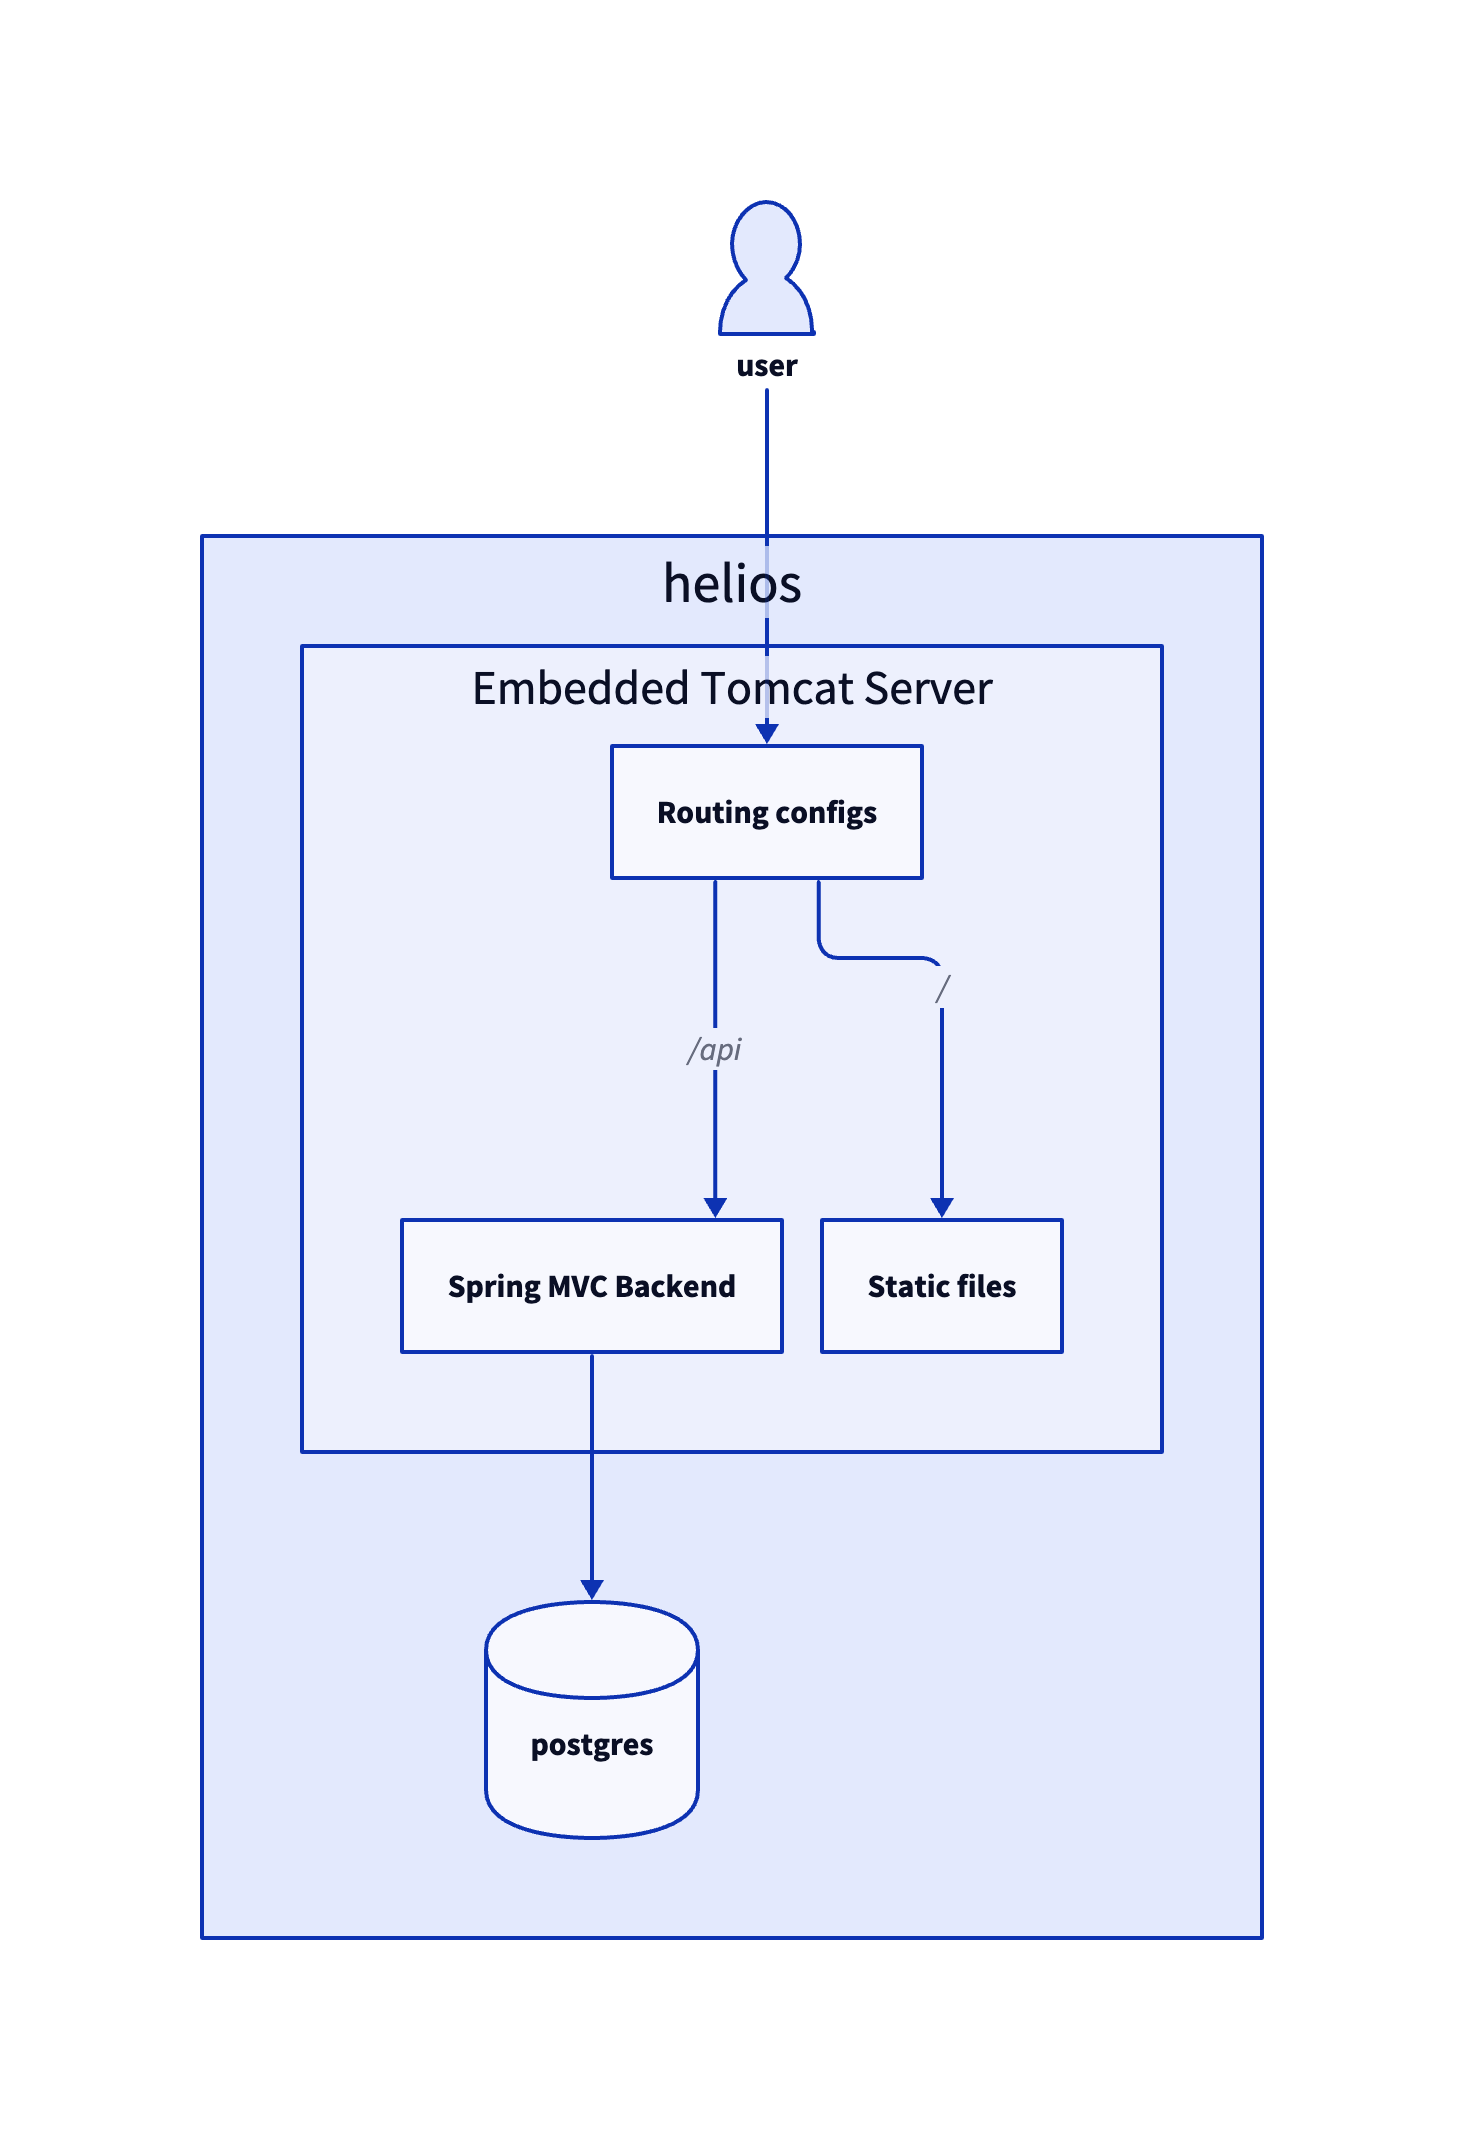
\includegraphics[width=0.5\textwidth]{./figures/architecture.png}
  \caption{Диаграмма архитектуры}\label{fig:arch}
\end{figure}


\printnoidxglossaries
\end{document}
